\documentclass[10pt]{beamer}

\usetheme{m}
\usepackage{lipsum}

\newcommand\blfootnote[1]{%
	\begingroup
	\renewcommand\thefootnote{}\footnote{#1}%
	\addtocounter{footnote}{-1}%
	\endgroup
}

\usepackage{booktabs}
\usepackage[scale=2]{ccicons}

\usepackage{pgfplots}
%\usepgfplotslibrary{dateplot}

\title{The dynamics and regulators of cell fate decisions are revealed by pseudotemporal ordering of single cells}
\subtitle{ Trapnell, Cole, et al (Nature biotechnology,2014)}
\date{\today}
\author{Saket Choudhary}
%\institute{Institute or miscellaneous information}
% \titlegraphic{\hfill
\includegraphics[height=1.5cm]{logo/logo}}

\begin{document}

\maketitle

%\begin{frame}
%  \frametitle{Table of Contents}
%  \setbeamertemplate{section in toc}[sections numbered]
%  \tableofcontents[hideallsubsections]
%\end{frame}

\section{Introduction}

\begin{frame}[fragile]
  \frametitle{rna-seq}
  \begin{itemize}[<+- | alert@+>]
\item rna-seq involved \emph{direct} sequencing of transcripts
\item Resolution at the level of individual isoform of genes
\item Area with ample scope of insights: biological and computational(RNA-Seq is \emph{challenging!})
\item  NOTE(A common misbelief): RNA-Seq doesn't measure what is \emph{technically} gene expression: Measures \emph{relative transcript abundances }
  \end{itemize}
  

  \blfootnote{Pachter, Lior. "Models for transcript quantification from RNA-Seq." arXiv preprint arXiv:1104.3889 (2011).}
\end{frame}


\begin{frame}[fragile]
	%\frametitle{RNA-Seq}
	\begin{figure}
		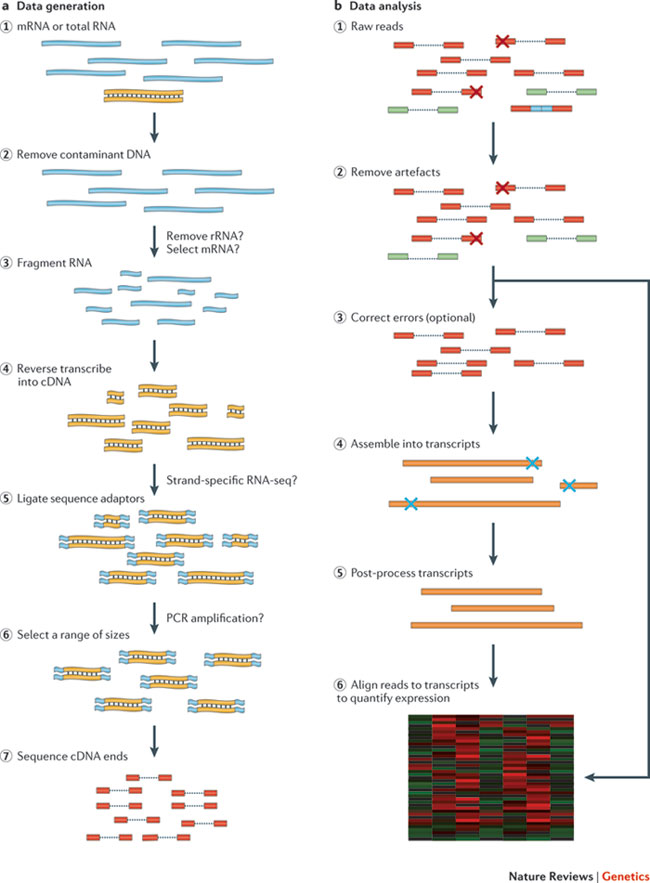
\includegraphics[scale=0.25]{images/rnaseq}
		\caption{ \footnotesize{A typical RNA-Seq experiment}}
	\end{figure}
	\vspace*{-26pt}
	\footnote{ {Next-generation transcriptome assembly, \emph{Martin et al. Nature Reviews Genetics(2011)}}}
	
	
\end{frame}


\begin{frame}[fragile]
	\frametitle{{Single cell rna-seq} Motivation}'
	Context: Studying differentiation
	
	 Transcriptional dynamics of a temporal process like cell differentiation is challenging
	\begin{itemize}[<+- | alert@+>]
		\item Time-series analysis of bulk cell data : hard to distinguish early and late phases of transcriptional cascade
		\item Difficult to capture cell-to-cell variability
	\end{itemize}
	\pause
	High variability arises due to high cell-to-cell variability: Simple averages don't work!

\end{frame}

\begin{frame}[fragile]
	\frametitle{Digression}
	Which is a better treatement?
	
	Treatments for kidney stones
	
	\begin{tabular}{|c|c|c|}
		\hline  & Treatment A  & Treatment B  \\ 
		\hline Small Stones & Group1: \textbf{93\%(81/87) } & Group2: 87\% (234/270)  \\ 
		\hline Large Stones & Group3: \textbf{73\%(192/263)} & Group 4
		69\% (55/80)  \\ 
		\hline 
	\end{tabular}
	\pause
	
	Hint: Is your sample size \emph{enough} to draw causality relations? 

\end{frame}


\begin{frame}[fragile]
	\frametitle{Digression}
	Which is a better treatement?
	
	Treatments for kidney stones
	
	\begin{tabular}{|c|c|c|}
		\hline  & Treatment A  & Treatment B  \\ 
		\hline Small Stones & Group1: \textbf{93\%(81/87) } & Group2: 87\% (234/270)  \\ 
		\hline Large Stones & Group3: \textbf{73\%(192/263)} & Group 4
		69\% (55/80)  \\ 
		\hline Both & 78\% (273/350) &	\textbf{83\% (289/350)} \\ 
		\hline 
	\end{tabular} 
	
	Reversal of inequality! : Simpson's Paradox. 
	Sizes of the groups being combined are not same. Large stones patients were offered \emph{better} treatment A, small stones patients were offered treatment B. $\implies$	Stone size is a 'confounding variable'.
	
\end{frame}


\section{Method}

\begin{frame}[fragile]
	\frametitle{Hypothesis}
	\begin{itemize}[<+- | alert@+>]
		\item RNA-Seq experiment constitutes a time-series: each cell is a discrete time point (during its differentiation)
		\item Using an unsupervised algorithm 'Monocle', we want to study the temporal development of single cell
		\item Cell type: Skeletal myoblasts $\implies$ known to undergo well-characterised sequence of transcriptional changes
		\item Cultured in high serum medium, then shifted to low serum $\implies$ induces differentiation 
	\end{itemize}
\end{frame}

\begin{frame}[fragile]
	\frametitle{Experiment}
	\begin{figure}
		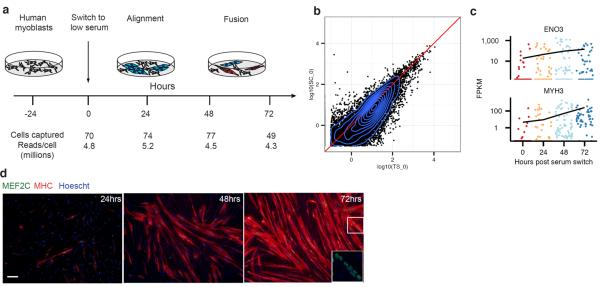
\includegraphics{images/expt1}
		\caption{a. Cell Culturing b. Sanity check with bulk RNA-seq(time=0) c.Late stage differentiation markers d. }
	\end{figure}
\end{frame}


\begin{frame}[fragile]
	\frametitle{Experiment}
	\begin{itemize}[<+- | alert@+>]
		\item Sanity Check: Single Cell rna-seq should correlate with bulk
		\item \emph{Known} markers such as ENO3, MYH3 are known to show increased expression with time
	\end{itemize}
\end{frame}

\begin{frame}[fragile]
	\frametitle{Methods}
	\begin{itemize}[<+- | alert@+>]
		\item Expression profile $\implies$ Represented as points in Euclidean space $\mathbb{R}^d$ where $d$ is the number of genes
		\item Reduce dimension: Independent Component Analysis:  Like PCA, but rather than maximising the variance, the projection ensures that the resulting data is one of the independent components of the data(Orthogonality still holds) 
		\item Construct a Minimum Spanning Tree using these points in 2D.
		\item Find the longest path through the MST which corresponds to the long-sequence of transcriptionally similar cells(Essentially with non significant differential expression )
		\item It is possible to create a trajectory using \emph{pseudotime} values: So there are now branches + a main trajectory(ref figure)
	\end{itemize}
\end{frame}


\begin{frame}[fragile]	
	%\frametitle{Method/Results}
	\begin{figure}
		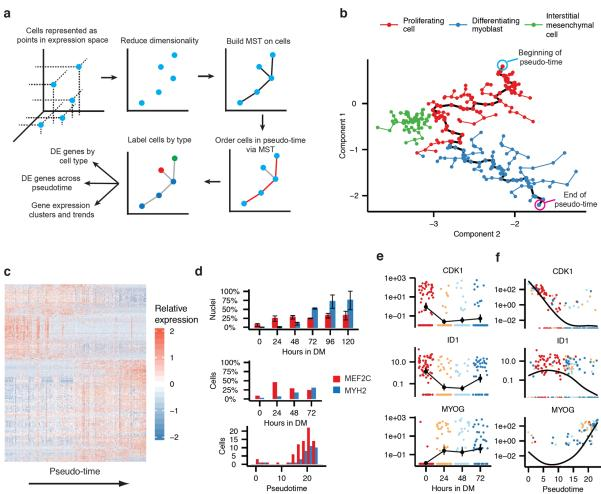
\includegraphics{images/expt2}
		\caption{Results}
	\end{figure}
\end{frame}


\section{Results}

\begin{frame}[fragile]	
	\frametitle{Method/Results}
	\begin{itemize}
		\item Differentiation = Two phase trajectory(differentiating) + non-differentiating cells
		\item Trajectory 1: Cells selected under High Mitogen Condition(Mitogen enhances differentiation/division)(time = 0 cells)
		\item Trajectory 2: 24h, 46h, 72h differentiating cells (MYOG is a known marker for differentiation)
		\item Trajectory 3: Lacks myogenic markers, possibly did not originate from the myoblasts(known to be stimulants of muscle differentiation) 
	\end{itemize}
\end{frame}

\begin{frame}[fragile]	
	\frametitle{Method/Results}
	\begin{figure}
		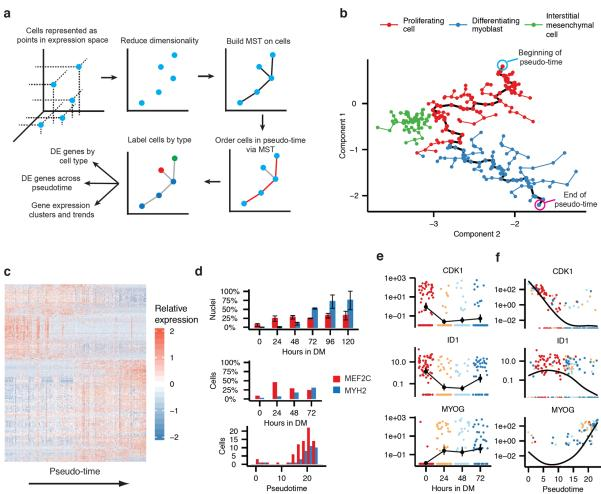
\includegraphics{images/expt2}
	\end{figure}
\end{frame}

\begin{frame}
	\frametitle{Results}
	\begin{itemize}[<+- | alert@+>]
		

	\item Sanity Check: Since the collection happened at 24h, 48h. 72h, it is possible to track the expression levels of markers: MEF2C, MYH2 by immunofluorescence and then compare it with pseudotime trajectory (ref Fig (d))
	\item Outcome: Monocle enables reconstructing the temporal trajectory of differentiation while retaining the in vitro differentiation kinetics 
	\item New Insight: Find differentially expressed genes that would otherwise have been
	 \emph{lost} in bulk RNA-seq: 	
	 
	 \end{itemize}
	 \pause
	 General Additive models:
	$$
	g(E(y)) = \beta_0 + f_1(x_1) + f_2(x_2) + \dots + f_m(x_m)
	$$
	where $x_i$ are the predictor variables. and $g$ is link function(log/identity) and $Y$ belong to the exponential family, the advantage over GLM being flexibility with nonparametric fits. (ofcourse, less interpretable than GLM)
\end{frame}

\begin{frame}
	\frametitle{More Validation}

\begin{itemize}
	\item A further validation step involved \emph{clustering} genes with \emph{[similar] } expression levels, with the assumption \textbf{similar trends in expression = similar biological function }
	\item Genes downregulated early or upregulated late were found to be GO enriched in myosis, cell cycle-exit, activation of muscle specific proteins
\end{itemize}


\end{frame}


\begin{frame}
		\frametitle{More Validation}
		\begin{figure}
			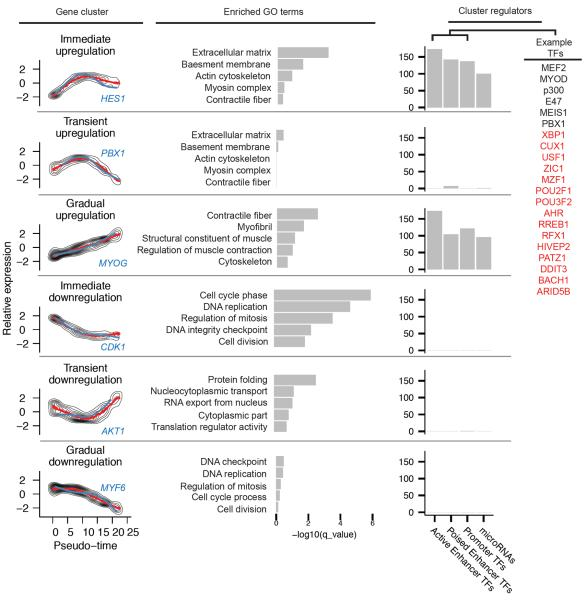
\includegraphics[scale=0.72]{images/expt3}
			\caption{GO analysis of gene clusters}
		\end{figure}
\end{frame}

\section{Conclusion}

\begin{frame}{Summary}

\begin{itemize}
	\item Monocle takes an unsupervised approach to determine the temporal trajectory for differentiating cells
	\item Makes it possible to identify the \emph{latent variables} that often get shadwoed with bulk RNA-Seq studies
	\item The GO validation step is not very convincing, the method otherwise looks solid(there were more experimental validations performed)
\end{itemize}
 
 \blfootnote{Yanai, Itai, et al. "Similar gene expression profiles do not imply similar tissue functions." TRENDS in Genetics 22.3 (2006): 132-138.}

\end{frame}

\plain{Questions?}



\end{document}
